\section{Methods}
\subsection{Parallel methods}
There are several granularities and ways of parallelization in this kind of 
Monte Carlo simulation. In the following, the used parallelization points and
its implementations are listed:

\begin{description}

  \item[Sample points] (multiple GPUs)\\
    The sample points introduced in \ref{subsec:meshSampling} are independent from each other
    and therefore its $\Phi$-ASE can be calculated in parallel. Every $\Phi$-ASE
    calculation runs in his own GPU-Kernel, thus sample points can be partioned 
    to several devices. As a result the speedup for multiple GPUs is almost linear.

  \item[Rays] (GPU threads)\\
    Every ray can be traced independently through the mesh structure.
    Exploiting this parallelism provides a great opportunity to boost
    performance. Only the resulting gains for each sample point have to be
    added atomatically in the end.
    Furthermore rays with same origin and direction will be grouped
    into warps to utilize the GPU cache in a good way.

  \item[Wavelengths] (Seperate block dimension)\\
    According to \ref{subsec:monteCarlo}, the simulation of a polychromatic
    laser can be split into sufficiently small monochromatic simulations which
    are again completely independent from each other.

\end{description}

\subsection{Importance sampling}
Importance sampling is a well known technique in the domain
of statistics \cite{importanceSamplingSource}. In case of 
ASE-Flux calculation a presampling of a sample point is done
to figure out which areas inside the mesh are worth to start rays from.
This method has a strong impact on the precision of the
simulation.

Figure \ref{graphic:importance} demonstrates
the differences between calculation with und without
importance sampling. It is shown each a cut through the activ 
gain medium in which the graphic without important
sampling has some peaks. Thus importance 
sampling can increase the efficiency of Monte-Carlo-Simulations 
by reducing variance and simulation runtime. 
\begin{figure}
  \centerline
  {\resizebox{0.45\textwidth}{!}{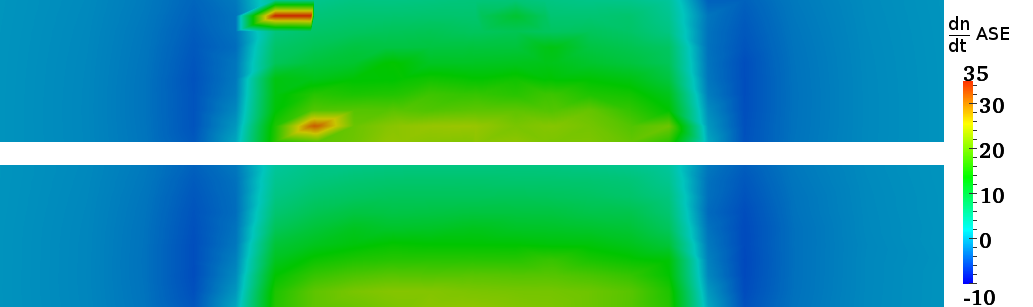
\includegraphics{graphics/importance.png}}}
  \caption{Cuts through activ gain medium: no importance sampling (top), with importance sampling (bottom)}
  \label{graphic:importance}
\end{figure}

\subsection{Adaptive sampling}
Since most sample points behave in a good way, there is no need
to sample them with a high number of rays. Only some outliers need to
be simulated with a higher precision. You can quantify the precision
and therefore the difference between the true and calculated value by
further determine the mean squared error (MSE).
The adaptive method allows you to remove strong peaks in the result
of the simulation without sampling all sample points with
a high number of rays and therefore reduce runtime.
\begin{figure}
  \centerline{
    \resizebox{0.45\textwidth}{!}{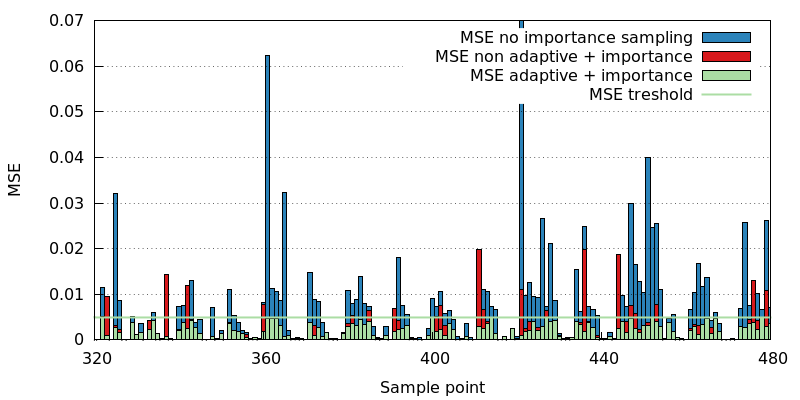
\includegraphics{plot/mse.png}}}
  \caption{Comparision no importance samling, not adaptive, adaptive}
  \label{plot:adaptive}
\end{figure}

In Figure~\ref{plot:adaptive} the adaptive method with 
50K to 500M rays per sample point is compared to the simulations
not adaptive and no importance sampling with each 300K rays per sample point (same runtime of 10s).
The not adaptive and no importance sampling method have some big peaks while all sample points of 
the adaptive method lie under a preset $MSE$-threshold (in this case 0.005). 

The adaptive method won't reduce the average MSE over sample points,
but it will reduce the maximal MSE values. Thus using the adaptives
methods gives higher precision by same calculation time.

%\begin{itemize}
%\item []
%     \[f(\vec{r_0}) = \frac{1}{n} \sum_{i=1}^n g_i \]
%     \[f^2(r_0) = \frac{1}{n} \sum_{i=1}^n g_i^2 \]
%     \[MSE(r_0) = \sqrt{\frac{f^2(r_0) - f(r_0)^2}{n}}\]
%\end{itemize}

